\documentclass[letterpaper]{article}

\usepackage[bottom=1cm, right=1cm, left=1cm, top=1cm]{geometry}
\pagenumbering{gobble}

\usepackage{multirow}
\usepackage{makecell}

\usepackage{musixtex}
\usepackage{gchords}
\usepackage{tikz}

\def\musicintext#1{
  {\let\extractline\relax
   \nobarnumbers
   \staffbotmarg0pt
   \startextract\addspace{-\afterruleskip}#1\endextract}}

\begin{document}

{
\centering
\begin{tabular}{ p{3cm} p{1.1cm} p{3.15cm} p{1.55cm} p{4.25cm} p{1.6cm} p{1.9cm} }
    \multicolumn{7}{c}{\Huge{Jazz Chords in C}} \\
    \hline
        \makecell[cl]{
            Minor Seventh} &
        \makecell[cl]{
            Cm\textsuperscript{7} \\
            C\textendash\textsuperscript{7} \\
            Cmi\textsuperscript{7} \\
            Cmin\textsuperscript{7}} &
        \makecell[cl]{
            Minor Seventh \\
            Minor Triad} &
        \makecell[cc]{
            \raisebox{0ex}[5ex][1ex]{
                \musicintext{\staffbotmarg2\Interligne
                \Notes \zw c\zw e\zw g\en}}} &
        \makecell[cc]{
            \begin{tikzpicture}
                \node{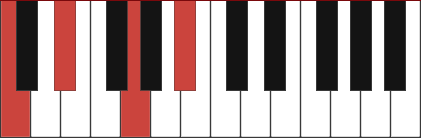
\includegraphics[width=0.2\textwidth]{assets/cm7.png}};
            \end{tikzpicture}} &
        \makecell[cl]{
            \chord{t}{n,f3p3,f2p2,n,f1p1,n}{}} & \\
    \hline
        \makecell[cl]{
            Dominant Seventh} &
        \makecell[cl]{
            C\textsuperscript{7}} &
        \makecell[cl]{
            Minor Seventh \\
            Major Triad} &
        \makecell[cc]{
            \raisebox{0ex}[5ex][1ex]{
                \musicintext{\staffbotmarg2\Interligne
                \Notes \zw c\zw e\zw g\en}}} &
        \makecell[cc]{
            \begin{tikzpicture}
                \node{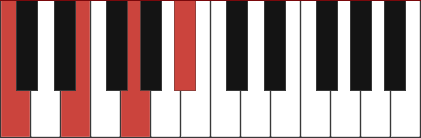
\includegraphics[width=0.2\textwidth]{assets/c7.png}};
            \end{tikzpicture}} &
        \makecell[cl]{
            \chord{t}{n,f3p3,f2p2,n,f1p1,n}{}} & \\
    \hline
        \makecell[cl]{
            Major Seventh} &
        \makecell[cl]{
            C\textsuperscript{maj7} \\
            C$\Delta$\textsuperscript{7} \\
            Cma\textsuperscript{7} \\
            CM\textsuperscript{7}} &
        \makecell[cl]{
            Major Seventh \\
            Major Triad} &
        \makecell[cc]{
            \raisebox{0ex}[5ex][1ex]{
                \musicintext{\staffbotmarg2\Interligne
                \Notes \zw c\zw e\zw g\zw i\en}}} &
        \makecell[cc]{
            \begin{tikzpicture}
                \node{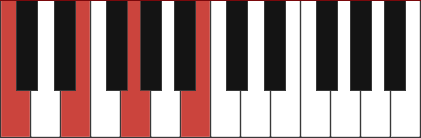
\includegraphics[width=0.2\textwidth]{assets/cmaj7.png}};
            \end{tikzpicture}} &
        \makecell[cl]{
            \chord{t}{n,f3p3,f2p2,n,f1p1,n}{}} & \\
    \hline
        \makecell[cl]{
            Major Sixth} &
        \makecell[cl]{
            C\textsuperscript{6}} &
        \makecell[cl]{
            Major Sixth \\
            Major Triad} &
        \makecell[cc]{
            \raisebox{0ex}[5ex][1ex]{
                \musicintext{\staffbotmarg2\Interligne
                \Notes \zw c\zw e\zw g\en}}} &
        \makecell[cc]{
            \begin{tikzpicture}
                \node{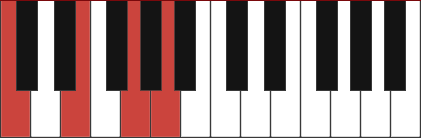
\includegraphics[width=0.2\textwidth]{assets/c6.png}};
            \end{tikzpicture}} &
        \makecell[cl]{
            \chord{t}{n,f3p3,f2p2,n,f1p1,n}{}} & \\
    \hline
        \makecell[cl]{
            Diminished} &
        \makecell[cl]{
            C\textsuperscript{o} \\
            Cdim} &
        \makecell[cl]{
            Diminished Fifth \\
            Minor Third \\
            Root} &
        \makecell[cc]{
            \raisebox{0ex}[5ex][1ex]{
                \musicintext{\staffbotmarg2\Interligne
                \Notes \zw c\zw e\zw g\en}}} &
        \makecell[cc]{
            \begin{tikzpicture}
                \node{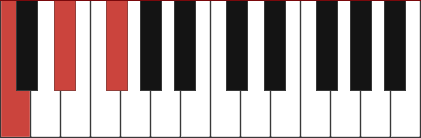
\includegraphics[width=0.2\textwidth]{assets/cdim.png}};
            \end{tikzpicture}} &
        \makecell[cl]{
            \chord{t}{n,f3p3,f2p2,n,f1p1,n}{}} & \\
    \hline
        \makecell[cl]{
            Fully Diminished \\
            Seventh} &
        \makecell[cl]{
            C\textsuperscript{o7} \\
            Cdim\textsuperscript{7}} &
        \makecell[cl]{
            Diminished Seventh \\
            Diminished} &
        \makecell[cc]{
            \raisebox{0ex}[5ex][1ex]{
                \musicintext{\staffbotmarg2\Interligne
                \Notes \zw c\zw e\zw g\en}}} &
        \makecell[cc]{
            \begin{tikzpicture}
                \node{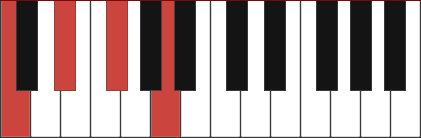
\includegraphics[width=0.2\textwidth]{assets/cdim7.png}};
            \end{tikzpicture}} &
        \makecell[cl]{
            \chord{t}{n,f3p3,f2p2,n,f1p1,n}{}} & \\
    \hline
        \makecell[cl]{
            Half Diminished \\
            Seventh} &
        \makecell[cl]{
            C\textsuperscript{\o{}7} \\
            Cm\textsuperscript{7$\flat$5} \\
            C\textendash\textsuperscript{7$\flat$5}} &
        \makecell[cl]{
            Minor Seventh \\
            Diminished} &
        \makecell[cc]{
            \raisebox{0ex}[5ex][1ex]{
                \musicintext{\staffbotmarg2\Interligne
                \Notes \zw c\zw e\zw g\en}}} &
        \makecell[cc]{
            \begin{tikzpicture}
                \node{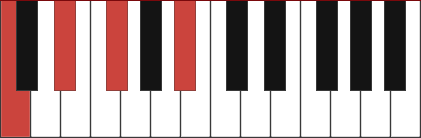
\includegraphics[width=0.2\textwidth]{assets/cm7b5.png}};
            \end{tikzpicture}} &
        \makecell[cl]{
            \chord{t}{n,f3p3,f2p2,n,f1p1,n}{}} & \\
    \hline
        \makecell[cl]{
            Minor Ninth} &
        \makecell[cl]{
            Cm9} &
        \makecell[cl]{
            Major Ninth \\
            Minor Seventh} &
        \makecell[cc]{
            \raisebox{0ex}[5ex][1ex]{
                \musicintext{\staffbotmarg2\Interligne
                \Notes \zw c\zw e\zw g\en}}} &
        \makecell[cc]{
            \begin{tikzpicture}
                \node{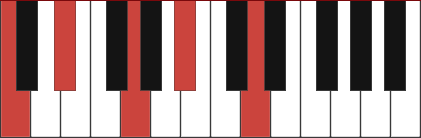
\includegraphics[width=0.2\textwidth]{assets/cm9.png}};
            \end{tikzpicture}} &
        \makecell[cl]{
            \chord{t}{n,f3p3,f2p2,n,f1p1,n}{}} & \\
    \hline
        \makecell[cl]{
            Dominant Ninth} &
        \makecell[cl]{
            C9} &
        \makecell[cl]{
            Major Ninth \\
            Dominant Seventh} &
        \makecell[cc]{
            \raisebox{0ex}[5ex][1ex]{
                \musicintext{\staffbotmarg2\Interligne
                \Notes \zw c\zw e\zw g\en}}} &
        \makecell[cc]{
            \begin{tikzpicture}
                \node{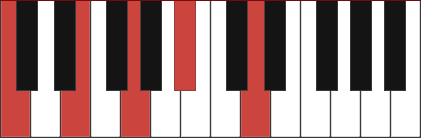
\includegraphics[width=0.2\textwidth]{assets/c9.png}};
            \end{tikzpicture}} &
        \makecell[cl]{
            \chord{t}{n,f3p3,f2p2,n,f1p1,n}{}} & \\
    \hline
        \makecell[cl]{
            Major Ninth} &
        \makecell[cl]{
            Cmaj9} &
        \makecell[cl]{
            Major Ninth \\
            Major Seventh} &
        \makecell[cc]{
            \raisebox{0ex}[5ex][1ex]{
                \musicintext{\staffbotmarg2\Interligne
                \Notes \zw c\zw e\zw g\en}}} &
        \makecell[cc]{
            \begin{tikzpicture}
                \node{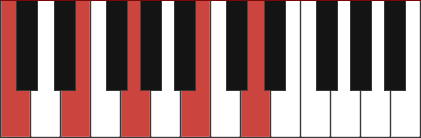
\includegraphics[width=0.2\textwidth]{assets/cmaj9.png}};
            \end{tikzpicture}} &
        \makecell[cl]{
            \chord{t}{n,f3p3,f2p2,n,f1p1,n}{}} & \\
    \hline
        \makecell[cl]{
            Eleventh} &
        \makecell[cl]{
            C11} &
        \makecell[cl]{
            Perfect Eleventh \\
            Major Ninth} &
        \makecell[cc]{
            \raisebox{0ex}[5ex][1ex]{
                \musicintext{\staffbotmarg2\Interligne
                \Notes \zw c\zw e\zw g\en}}} &
        \makecell[cc]{
            \begin{tikzpicture}
                \node{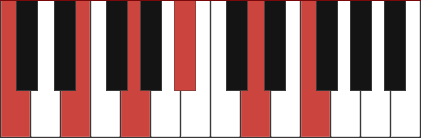
\includegraphics[width=0.2\textwidth]{assets/c11.png}};
            \end{tikzpicture}} &
        \makecell[cl]{
            \chord{t}{n,f3p3,f2p2,n,f1p1,n}{}} &
        \makecell[cl]{
            Omit third
        } \\
    \hline
        \makecell[cl]{
            Thirteenth} &
        \makecell[cl]{
            C13} &
        \makecell[cl]{
            Major Thirteenth \\
            Dominant Ninth} &
        \makecell[cc]{
            \raisebox{0ex}[5ex][1ex]{
                \musicintext{\staffbotmarg2\Interligne
                \Notes \zw c\zw e\zw g\en}}} &
        \makecell[cc]{
            \begin{tikzpicture}
                \node{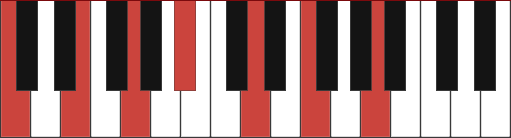
\includegraphics[width=0.2\textwidth]{assets/c13.png}};
            \end{tikzpicture}} &
        \makecell[cl]{
            \chord{t}{n,f3p3,f2p2,n,f1p1,n}{}} & \\
    \hline
        \makecell[cl]{
            Augmented} &
        \makecell[cl]{
            C\textsuperscript{+} \\
            Caug \\
            C\textsuperscript{$\sharp$5}} &
        \makecell[cl]{
            Augmented Fifth \\
            Major Third \\
            Root} &
        \makecell[cc]{
            \raisebox{0ex}[5ex][1ex]{
                \musicintext{\staffbotmarg2\Interligne
                \Notes \zw c\zw e\zw g\en}}} &
        \makecell[cc]{
            \begin{tikzpicture}
                \node{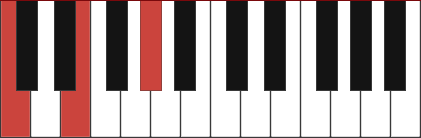
\includegraphics[width=0.2\textwidth]{assets/caug.png}};
            \end{tikzpicture}} &
        \makecell[cl]{
            \chord{t}{n,f3p3,f2p2,n,f1p1,n}{}} & \\
    \hline
\end{tabular}\par
}

\end{document}